	\section{Sunetul}
	Sunetul reprezint\u{a} vibra\c{t}ia undelor propagate \^{i}ntr-un mediu, fie el gazos, lichid sau solid \c{s}i prezint\u{a}, \^{i}n multe aspecte, dar nu \^{i}n toate, comportament similar cu alte mi\c{s}c\u{a}ri de und\u{a} pe care le \^{i}nt\^{a}lnim \^{i}n natur\u{a}, adic\u{a} undele de ap\u{a} \c{s}i undele de lumin\u{a}, ale c\u{a}ror fenomene de propagare sunt u\c{s}or de
	observat.
	 
	
	\^{I}n contextul propag\u{a}rii sunetului, aerul este mediul de interes despre care vom discuta atunci c\^{a}nd vorbim despre acustica \^{i}nc\u{a}perilor, iar perturbarea reprezint\u{a} o alterare a presiunii atmosferice peste \c{s}i sub valoarea sa medie, care produce o mi\c{s}care periodic\u{a} a moleculelor de aer \^{i}napoi \c{s}i \^{i}nainte de-a lungul aceleia\c{s}i direc\c{t}ii \^{i}n care se propag\u{a} unda (unde longitudinale).
	 
	
	Propagarea sunetului prin aer este ilustrat\u{a} în Figura \ref{Fig1}. \^{I}n partea superioar\u{a}
	este ilustrat\u{a} alterarea presiunii atmosferice, \^{i}n timp ce \^{i}n partea inferioar\u{a} este ilustrat\u{a} mi\c{s}carea moleculelor de aer asociate cu propagarea sunetului. Dac\u{a} intensitatea
	sunetului cre\c{s}te, gradientul presiunii cre\c{s}te \c{s}i, ca urmare, mai multe
	molecule de aer se afl\u{a} \^{i}n mi\c{s}care.
	
	\begin{figure}[!htb]
		\centering
		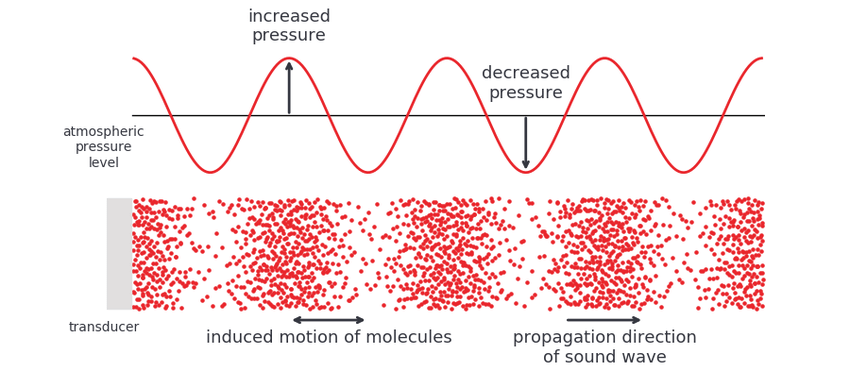
\includegraphics[width=1\linewidth]{imagini/propagareaSunetuluiInAer.png}
		\caption{Propagarea sunetului prin aer\cite{elorza}}
		\label{Fig1}
	\end{figure}

	Un principiu general, stabilit pentru prima dat\u{a} de Fermat, afirm\u{a} c\u{a} fiecare und\u{a} se propag\u{a} de la surs\u{a} c\u{a}tre receptor prin calea cea mai rapid\u{a}. Dac\u{a} mediul este omogen, precum consider\u{a}m c\u{a} este aerul, atunci viteza sunetului este uniform\u{a} prin acest mediu \c{s}i astfel calea cea mai rapid\u{a} devine totodat\u{a} \c{s}i cea mai scurt\u{a}.
	Viteza sunetului depinde doar de temperatur\u{a}, nu \c{s}i de alte propriet\u{a}\c{t}i precum presiunea \c{s}i densitatea. Astfel, putem observa \^{i}n Tabelul \ref{Tabel1} cum variaz\u{a} viteza \c{s}i densitatea sunetului \^{i}n func\c{t}ie de temperatur\u{a}.
	
	 
	\begin{table}[!htb]
		\centering		
	\begin{tabular}{|c|c|c|}
		\hline
		\bf{Temperatur\u{a} ($^{\circ}$C)} & \bf{Viteza sunetului $\left(\dfrac{m}{s} \right)$} & \bf{Densitatea aerului $\left(\dfrac{kg}{m^3}\right)$}\\
		\hline \hline
		
		30 & 349.02 & 1.1644\\
		\hline
		25 & 346.13 & 1.1839\\
		\hline
		20 & 343.21 & 1.2041\\
		\hline
		15 & 340.27 & 1.2250\\
		\hline
		10 & 337.31 & 1.2466\\
		\hline
		5 & 334.32 & 1.2690\\
		\hline
		0 & 331.30 & 1.2922\\
		\hline			
	\end{tabular}
	\caption{Efectul temperaturii asupra propriet\u{a}\c{t}ilor aerului\cite{temperaturaTabel}}
	\label{Tabel1}
	\end{table}

	{\it{Amplitudinea}} este valoarea absolut\u{a}, maxim\u{a}, a unei cantit\u{a}\c{t}i care variaz\u{a} periodic. Amplitudinile sunt exprimate fie ca valori instantanee, fie mai ales ca valori de v\^{a}rf. Aceasta reprezint\u{a} fluctua\c{t}ia sau deplasarea unei unde de la valoarea sa medie. \^{I}n cazul undelor sonore, particulele de aer sunt deplasate, iar aceast\u{a} amplitudine a sunetului este exprimat\u{a} ca intensitatea sunetului. Amplitudinea nu este influen\c{t}at\u{a} de frecven\c{t}\u{a}, de lungimea de und\u{a}, de perioada de timp sau de viteza sunetului \c{s}i nici invers.
	 
	{\it{Lungimea de und\u{a}}} este reprezentat\u{a} de distan\c{t}a dintre punctele consecutive corespunz\u{a}toare ale aceleia\c{s}i faze de und\u{a}, precum dou\u{a} creste adiacente. {\it{Viteza de propagare ($c$)}} a undei este dat\u{a} de lungimea de und\u{a}, pe care o vom nota cu $\lambda$, fiind distan\c{t}a parcurs\u{a} de val \^{i}ntre dou\u{a} instan\c{t}e de faz\u{a} egal\u{a} \c{s}i de timp, $T$, timpul necesar acestei distan\c{t}e.
	
	\begin{equation}
	c=\lambda/T
	\end{equation}
	 	
	Inversa perioadei este numit\u{a} {\it{frecven\c{t}\u{a} ($f$)}} \c{s}i indic\u{a} de c\^{a}te ori particulele de aer s-au mi\c{s}cat \^{i}napoi \c{s}i \^{i}nainte \^{i}ntr-o secund\u{a}. Frecven\c{t}a este m\u{a}surat\u{a} \^{i}n Hertz[Hz].
	
	\begin{equation}
	c=\lambda f
	\end{equation}	 
	
	O caracteristic\u{a} important\u{a} a unei unde sonore este {\it{faza}}, care specific\u{a} loca\c{t}ia unui punct \^{i}n cadrul unui ciclu de und\u{a} al unei forme de und\u{a} repetitive. \^{I}n majoritatea cazurilor, diferen\c{t}ele de faz\u{a} dintre undele sonore sunt mai importante dec\^{a} fazele \^{i}n sine. Diferen\c{t}a de faz\u{a} dintre dou\u{a} unde sonore cu aceea\c{s}i frecven\c{t}\u{a} care se deplaseaz\u{a} dincolo de o loca\c{t}ie fix\u{a} este dat\u{a} de diferen\c{t}a de timp dintre acelea\c{s}i pozi\c{t}ii \^{i}n cadrul ciclurilor de und\u{a} ale celor dou\u{a} sunete, exprimate ca o frac\c{t}iune dintr-un ciclu de und\u{a}. 	  
	
	Dou\u{a} unde sonore de aceea\c{s}i frecven\c{t}\u{a} care sunt perfect aliniate au o diferen\c{t}\u{a} de faz\u{a} de 0 \c{s}i se spune c\u{a} sunt ,,\^{i}n faz\u{a}". Dou\u{a} unde care sunt ,,\^{i}n faz\u{a}" se adaug\u{a} pentru a produce o und\u{a} sonor\u{a} cu o amplitudine egal\u{a} cu suma amplitudinilor celor dou\u{a} unde, precum în Figura \ref{Fig7}.

	\begin{figure}[!htb]
		\centering
		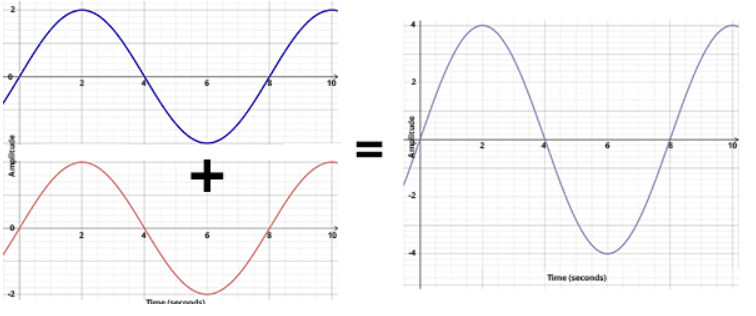
\includegraphics[width=10cm]{imagini/soundWaveGreaterAmplitude.png}
		\caption{Dou\u{a} unde sonore ,,\^{i}n faz\u{a}"}
		\label{Fig7}
	\end{figure}

	Dac\u{a} una dintre cele dou\u{a} unde sonore cu aceea\c{s}i frecven\c{t}\u{a} este deplasat\u{a} cu o jum\u{a}tate de ciclu fa\c{t}\u{a} de cealalt\u{a}, se spune c\u{a} undele sonore sunt ,,defazate". Dou\u{a} unde sunt ,,defazate" dac\u{a} se anuleaz\u{a} reciproc exact c\^{a}nd sunt adunate \^{i}mpreun\u{a}, precum în Figura \ref{Fig8}.

	\begin{figure}[!htb]
		\centering
		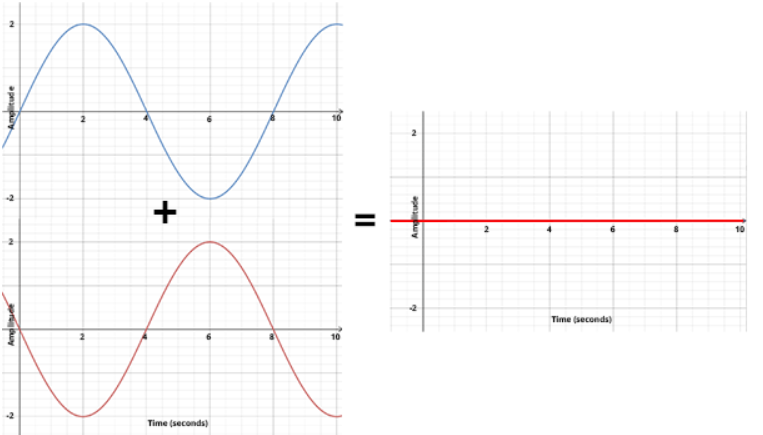
\includegraphics[width=10cm]{imagini/soundWaveCanceledAmplitude.png}
		\caption{Dou\u{a} unde sonore ,,defazate"}
		\label{Fig8}
	\end{figure}

	Diferen\c{t}a de faz\u{a} este exprimat\u{a} ca un unghi, deoarece forma de und\u{a} a unui ton pur alc\u{a}tuit\u{a} dintr-o singur\u{a} frecven\c{t}\u{a} poate fi descris\u{a} utiliz\^{a}nd func\c{t}ia sinus trigonometric\u{a}.	 
	
	Cele mai multe sunete sunt mult mai complexe dec\^{a}t o singur\u{a} frecven\c{t}\u{a}, dar constau \^{i}n schimb din multe unde sinusoidale diferite la frecven\c{t}e diferite. C\^{a}nd mai multe unde sinusoidale se combin\u{a} pentru a crea un sunet, formele de und\u{a} ale tuturor undelor sinusoidale sunt ad\u{a}ugate la fiecare loca\c{t}ie de-a lungul formei de und\u{a}.
	 	
	{\it{Energia (W)}} poate fi auzit\u{a} de fiin\c{t}ele vii. Sunetul este o und\u{a} mecanic\u{a} \c{s}i ca atare const\u{a} fizic \^{i}n compresie elastic\u{a} oscilatorie \c{s}i \^{i}n deplasarea oscilatorie a unui fluid. Prin urmare, mediul ac\c{t}ioneaz\u{a} ca stocare at\^{a}t pentru energia poten\c{t}ial\u{a}, c\^{a}t \c{s}i pentru energia cinetic\u{a}. \^{I}n consecin\c{t}\u{a}, energia sonor\u{a} dintr-un volum de interes este definit\u{a} ca suma densit\u{a}\c{t}ilor de energie poten\c{t}ial\u{a} \c{s}i cinetic\u{a}:
	
	\begin{equation}
	W = W_{\text{poten\c{t}ial\u{a}}} + W_{\text{cinetic\u{a}}}
	\end{equation}  
	
	{\it{Presiunea acustic\u{a}}} este abaterea presiunii locale fa\c{t}\u{a} de presiunea atmosferic\u{a}. \^{I}n aer, presiunea poate fi m\u{a}surat\u{a} cu ajutorul unui microfon, iar \^{i}n ap\u{a} cu ajutorul unui hidrofon. Unitatea de m\u{a}sur\u{a} dat\u{a} de c\u{a}tre Sistemul Interna\c{t}ional de Unit\u{a}\c{t}i de M\u{a}sur\u{a}, SI, pentru presiunea acustic\u{a} este Pascal (Pa). Formula folosit\u{a} pentru transformarea intensit\u{a}\c{t}ii \^{i}n presiune este:
	
	\begin{equation}
	p = \sqrt{2 I \rho c}, 
	\end{equation}
	
	\noindent unde $\rho$ este densitatea aerului, iar $c$ este viteza sunetului.	 
	
	{\it{Puterea sunetului}} este rata la care energia sonor\u{a} este emis\u{a}, reflectat\u{a}, transmis\u{a} sau recep\c{t}ionat\u{a}, pe unitate de timp. Unitatea SI pentru puterea sunetului este Watt-ul (W). Pentru o surs\u{a} de sunet, spre deosebire de presiunea sonor\u{a}, puterea nu este dependent\u{a} nici de \^{i}nc\u{a}pere, nici de distan\c{t}\u{a}. Presiunea sonor\u{a} este o proprietate a c\^{a}mpului \^{i}ntr-un punct din spa\c{t}iu, \^{i}n timp ce puterea sonor\u{a} este proprietatea unei surse sonore, egal\u{a} cu puterea total\u{a} emis\u{a} de acea surs\u{a} \^{i}n toate direc\c{t}iile.
	 	
	{\it{Intensitatea (I)}} este definit\u{a} ca putere pe unitate de suprafa\c{t}\u{a} purtat\u{a} de o und\u{a}. {\it{Puterea (P)}} este rata la care energia este transferat\u{a} de und\u{a}. Unitatea de m\u{a}sur\u{a} folosi\u{a} pentru intensitate este $\dfrac{W}{m^2}$, iar formula acesteia este:
	
	\begin{equation}
	I=\frac{P}{A}
	\end{equation}
	 	
	Intensitatea sunetului este măsurată și raportată în decibeli (dB), o unitate care exprimă magnitudinea relativă a unui sunet pe o scară logaritmică. {\it{Nivelurile de intensitate}} ale sunetului sunt citate în decibeli (dB). Modul în care urechile noastre percep sunetul poate fi descris mai exact prin logaritmul intensit\u{a}\c{t}ii. Nivelul de intensitate ($\beta$) este definit astfel:
	
	\begin{equation}
	\beta(dB) = 10 \lg\left(\dfrac{I}{I_0}\right) 
	\end{equation}

	Omul de știință folosește, în mod obișnuit, patru termeni pentru a descrie amploarea unei unde sonore, fiecare dintre acestea putând fi tradus într-o versiune echivalentă a celeilalte. Amplitudinea se concentrează pe dimensiunea vibrației particulelor, iar presiunea sonoră asupra forței pe care o astfel de vibrație o exercită asupra mediului înconjurător. Ceilalți doi termeni, intensitate și putere, pun accentul pe noțiunea mai abstractă a energiei undei, corelând-o astfel cu alte forme de transfer și schimb de energie.
	
	Una dintre caracteristicile fizice importante legate de propagarea sunetului este impedanță acustică a mediului în care se deplasează unda sonoră. \textit{Impedanța acustică} este dată de raportul dintre presiunea acustică a undei și viteza sa de volum.
	
	\section{Reflexia sunetului}
	
	Principiile reflexiei pot fi aplicate undelor sonore, care constau din compresii \c{s}i refrac\c{t}ii. Dac\u{a} o und\u{a} sonor\u{a} se deplaseaz\u{a} printr-un tub cilindric, \^{i}n cele din urm\u{a} sunetul va ajunge la cap\u{a}tul tubului, acesta reprezent\^{a}nd grani\c{t}a dintre aerul din tub \c{s}i aerul din afara tubului. La atingerea cap\u{a}tului tubului, unda sonor\u{a} va suferi o reflec\c{t}ie par\c{t}ial\u{a} (o parte din energia transportat\u{a} va r\u{a}m\^{a}ne \^{i}n tub \c{s}i se va deplasa \^{i}n direc\c{t}ia opus\u{a}) \c{s}i o transmisie par\c{t}ial\u{a} (o parte din energia transportat\u{a} va trece peste grani\c{t}\u{a}, \^{i}n afara tubului).
	 
	
	Reflexia pe suprafe\c{t}e poate duce la unul dintre urm\u{a}toarele fenomene: ecou sau reverbera\c{t}ie. {\it{Ecoul}} este o reflexie a sunetului care ajunge la ascult\u{a}tor cu o \^{i}nt\^{a}rziere fa\c{t}\u{a} de sunetul direct. Aceast\u{a} \^{i}nt\^{a}rziere este direct propor\c{t}ional\u{a} cu distan\c{t}a suprafe\c{t}ei reflectate de la surs\u{a} la ascult\u{a}tor. Undele acustice sunt reflectate de pere\c{t}i sau de alte suprafe\c{t}e dure, cum ar fi mun\c{t}ii. Ecoul poate fi auzit atunci c\^{a}nd reflexia revine cu o amplitudine \c{s}i o \^{i}nt\^{a}rziere suficient\u{a} pentru a fi perceput\u{a} distinct. 
	 
	
	{\it{Reverberarea}} reprezint\u{a} o persisten\c{t}\u{a} a sunetului dup\u{a} ce acesta a fost produs. O reverbera\c{t}ie este creat\u{a} atunci c\^{a}nd un sunet sau semnal provoac\u{a} multiple reflexii care se acumuleaz\u{a} \c{s}i apoi se descompun pe m\u{a}sur\u{a} ce sunetul este absorbit de suprafe\c{t}e. \^{I}n Figura \ref{Fig2}, observ\u{a}m dou\u{a} diagrame ce prezintă pe axa Ox, timpul, \c{s}i pe axa Oy, SPL (Sound Pressure Level) ce ilustreaz\u{a} diferen\c{t}a dintre ecou \c{s}i reverbera\c{t}ie. 
	
	\begin{figure}[!htb]
		\centering
		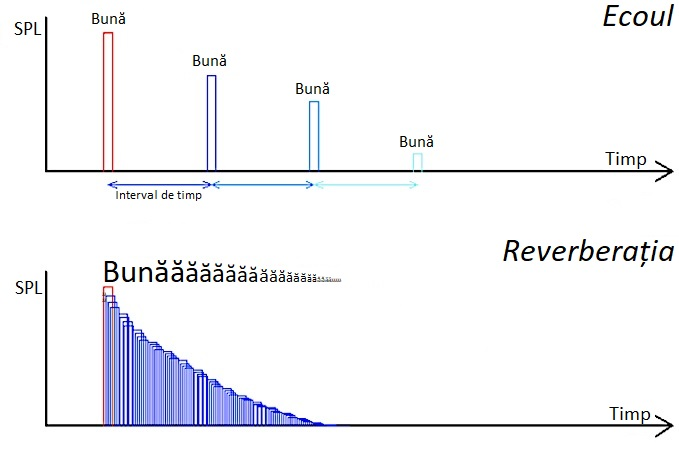
\includegraphics[width=1\linewidth]{imagini/EchoReverberation.jpg}
		\caption{Diferen\c{t}a dintre ecou \c{s}i reverbera\c{t}ie}
		\label{Fig2}
	\end{figure}

	Trasarea razelor pentru calcularea unghiurilor de inciden\c{t}\u{a} sau refrac\c{t}ie este dat\u{a} de legea lui Snell prin Ecua\c{t}ia \eqref{SnellEq} (vezi \cite{snell}):
	
	\begin{equation}
		\label{SnellEq}
		\frac{\sin \theta_2}{\sin \theta_1} = \frac{v_2}{v_1} = \frac{n_1}{n_2}
	\end{equation}

	\noindent unde $\theta_1, \theta_2$ sunt unghiurile de refrac\c{t}ie, $v_1, v_2$ reprezint\u{a} viteza de propagare prin mediu, iar $n_1, n_2$ sunt indicii de refrac\c{t}ie din mediu.
	
	\begin{figure}[!htb]
		\centering
		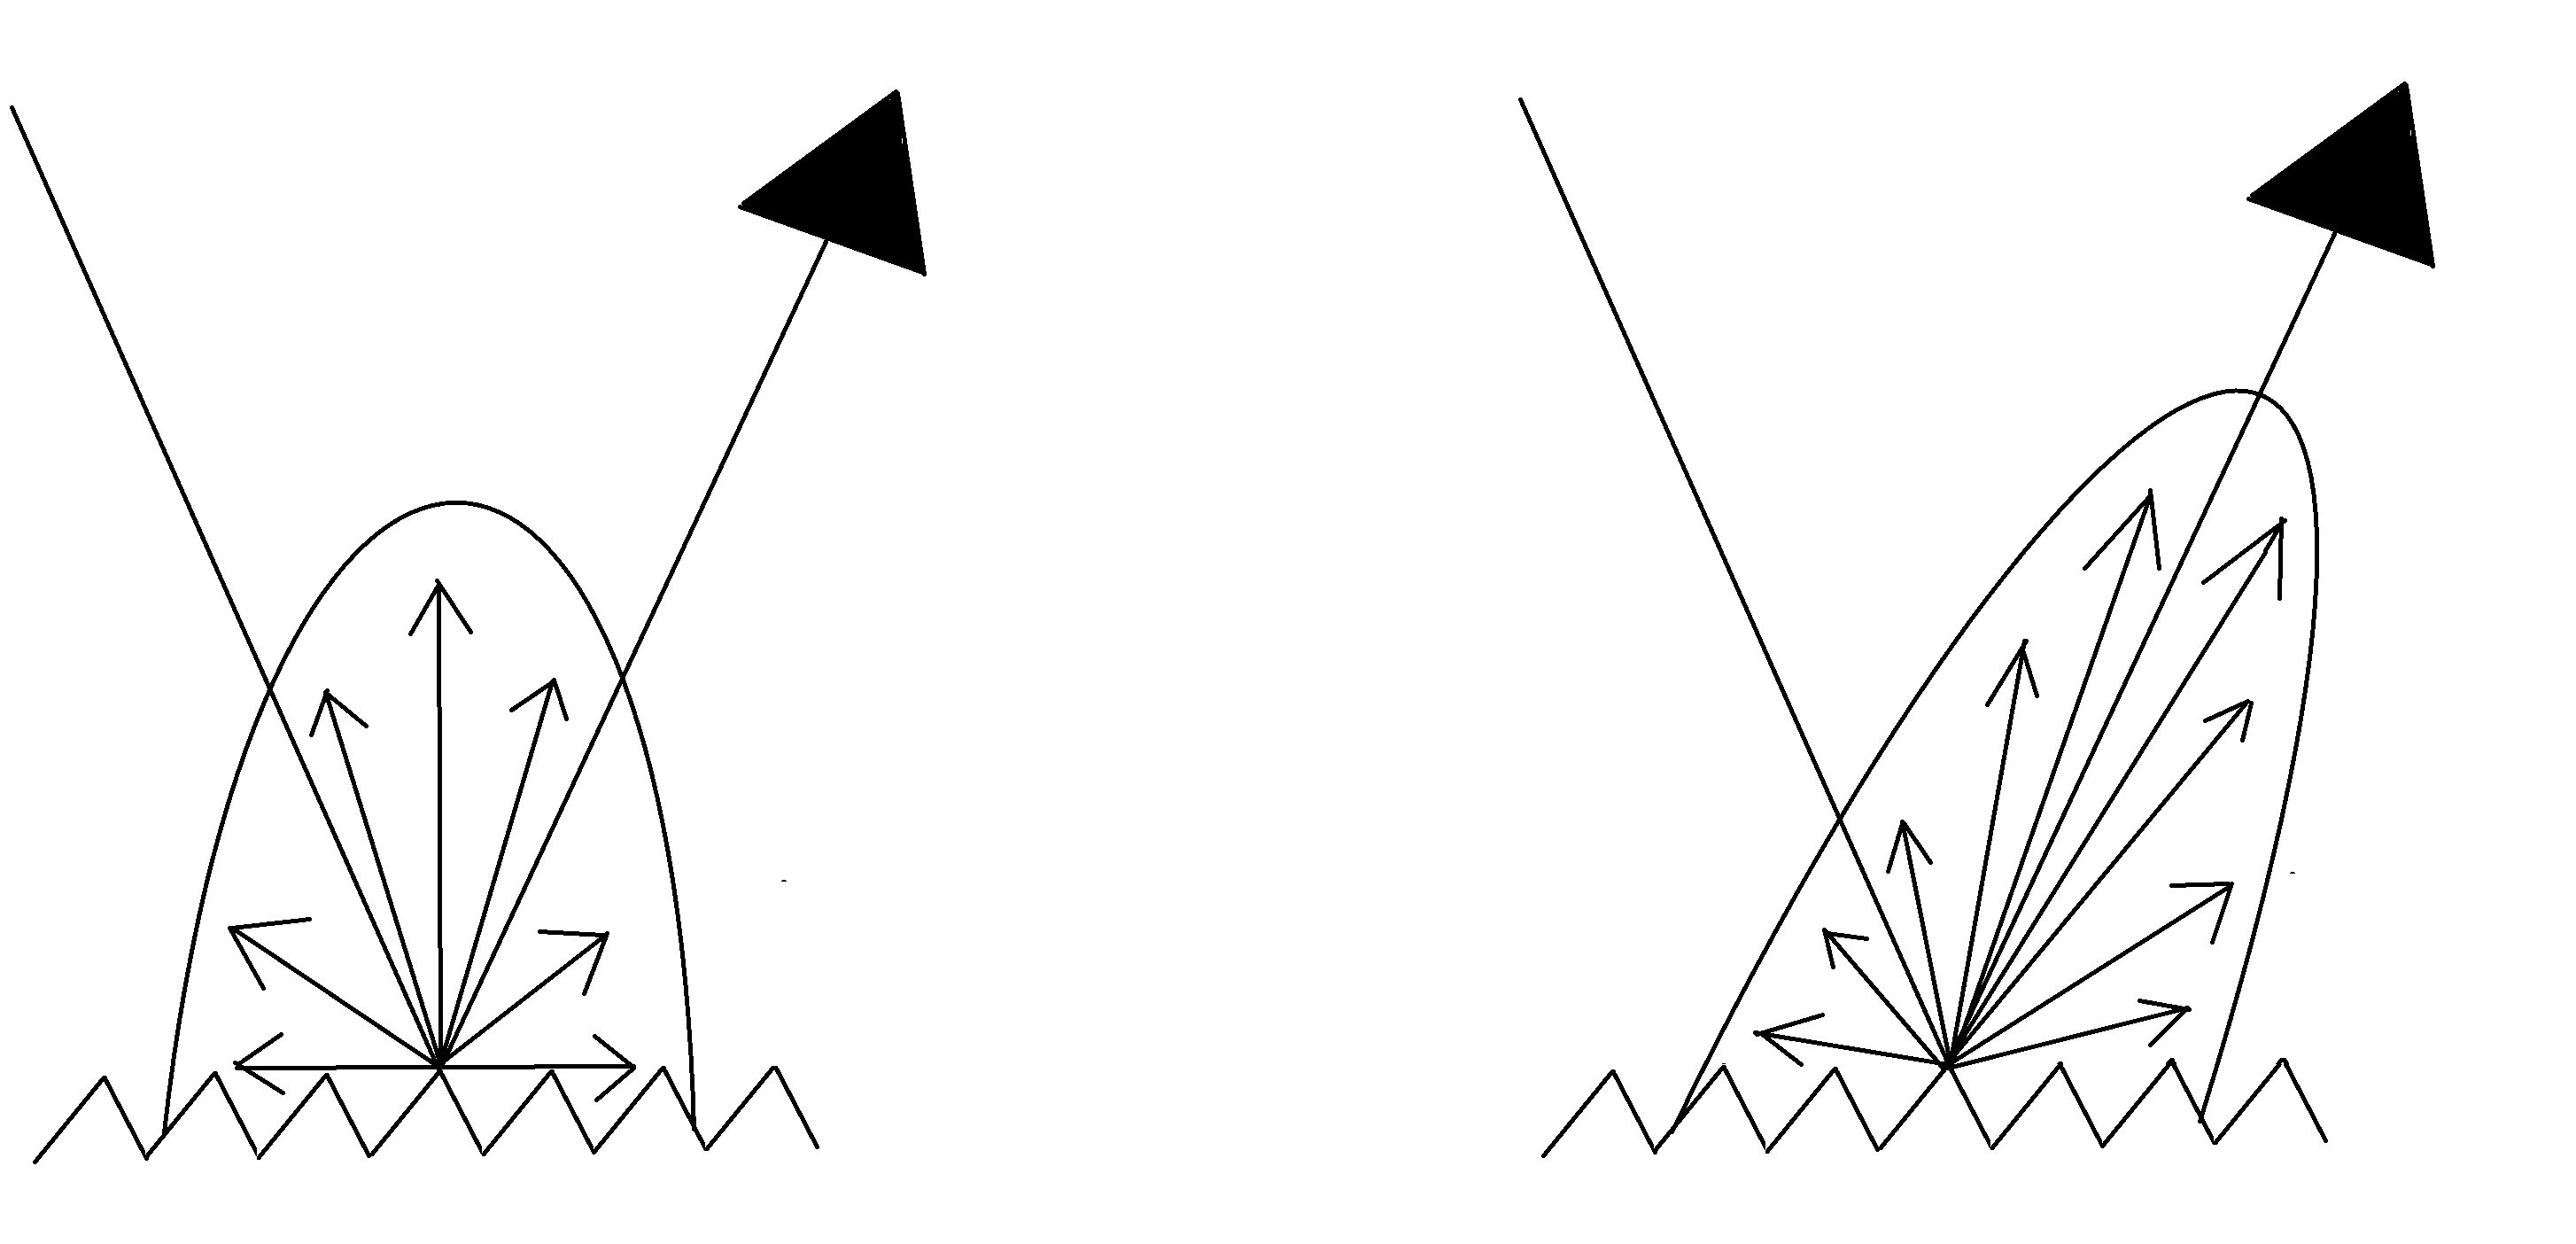
\includegraphics[width=0.7\linewidth]{imagini/reflections.png}
		\caption{Reflexie difuz\u{a} prin randomizare normal\u{a} \c{s}i reflexie difuz\u{a} prin randomizare ponderat\u{a}}
		\label{Fig10}
	\end{figure}

	Reflexiile sunetului pe suprafe\c{t}e nu urmeaz\u{a} \^{i}ntotdeauna legile lui Snell. Astfel, nici o reflexie nu este perfect specular\u{a}, deci este par\c{t}ial difuz\u{a}, iar acest lucru se \^{i}nt\^{a}mpl\u{a} ca o consecin\c{t}\u{a} pentru duritatea \c{s}i dimensiunea suprafe\c{t}ei de coliziune. Când o rază întâlnește o
	suprafață difuză, se generează un număr aleatoriu în intervalul [0, 1]. Dac\u{a} num\u{a}rul este mai mic dec\^{a}t un prag ales direc\c{t}ia razei este randomizat\u{a} pentru a simula difuzia, altfel	reflexia este specular\u{a}. Acest fenomen poate fi eviden\c{t}iat prin Figura \ref{Fig10}. \^{I}n aceast\u{a} lucrare se va folosi reflexia difuz\u{a} prin randomizare normal\u{a}.
	


	\section{Difrac\c{t}ia \c{s}i interferen\c{t}a sunetului}
	
	Difrac\c{t}ia reprezint\u{a} schimbarea local\u{a} \^{i}n direc\c{t}ia propag\u{a}rii undelor sonore trec\^{a}nd de marginea unui obstacol. Acesta este unul dintre cele mai importante fenomene acustice cauzat de natura sunetului, fiind una dintre cele mai complexe probleme de rezolvat. Efectele difrac\c{t}iei pot fi \^{i}mp\u{a}r\c{t}ite \^{i}n trei grupe: barier\u{a}, margine \c{s}i deschidere.
	 
	
	Fenomenul de difrac\c{t}ie depinde semnificativ de raportul dintre lungimea de und\u{a} a sunetului si m\u{a}rimea obstacolului. Cu c\^{a}t lungimea de und\u{a} este mai mare, cu at\^{a}t sunetul se intensific\u{a}. C\^{a}nd o und\u{a} sonor\u{a} \^{i}nt\^{a}lne\c{s}te un obstacol, care este mic \^{i}n raport cu lungimea de und\u{a}, valul trece \^{i}n jurul ei ca \c{s}i c\^{a}nd nu ar exista, form\^{a}nd foarte pu\c{t}in\u{a} umbr\u{a}. Dac\u{a} frecven\c{t}a sunetului este suficient de mare, lungimea de und\u{a} este suficient de scurt\u{a} \c{s}i ca urmare se formeaza\u{a} o umbr\u{a} vizibil\u{a}.
	 
	
	\^{I}n Figura \ref{Fig3} se pot observa cele trei tipuri de difrac\c{t}ii, unde situa\c{t}iile din partea de sus sunt ideale pentru frecven\c{t}ele joase, iar cazurile din partea de jos sunt de dorit pentru frecven\c{t}ele \^{i}nalte.
	 
	
	\begin{figure}[!htb]
		\centering
		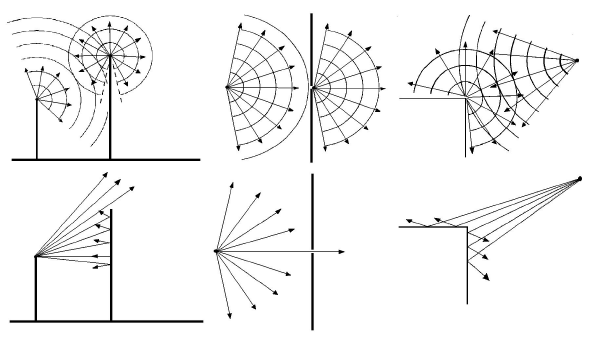
\includegraphics[width=0.8\linewidth]{imagini/difractie.png}
		\caption{Difrac\c{t}ie barier\u{a}, deschidere, margine\cite{elorza}}
		\label{Fig3}
	\end{figure}
	
	Dou\u{a} unde care c\u{a}l\u{a}toresc \^{i}n acela\c{s}i mediu vor interfera una cu cealalt\u{a}. Dac\u{a} amplitudinile lor se adun\u{a}, se spune c\u{a} aceasta este o interferen\c{t}\u{a} constructiv\u{a} și se află ,,în fază''. O interferen\c{t}\u{a} distructiv\u{a} se constituie din două unde ,,defazate'' și se realizeaz\u{a} atunci c\^{a}nd cele dou\u{a} unde sonore sunt defazate \c{s}i scad. Interferența constructivă duce la o creștere a amplitudinii undei, în timp ce interferența distructivă poate duce la anularea totală a undelor care contribuie.
	 
	Difracția sunetului este utilă în cazul sistemelor audio, în care sunetul provenit de la difuzoare se răspândește și se reflectă de pe pereți pentru a umple o cameră. Pe de altă parte, capacitatea unei unde sonore de a difracta scade pe măsură ce frecvența crește și lungimea de undă se micșorează. De asemenea, deoarece lungimile de undă ale semnalelor ultrasonice devin extrem de mici la frecvențe înalte, este posibil să se creeze un fascicul de ultrasunete. Fasciculele cu ultrasunete au devenit foarte utile în medicina modernă.
	
	\^{I}n acest studiu, difrac\c{t}ia nu va fi un subiect abordat.
	
	\section{Func\c{t}ia de r\u{a}spuns la impuls}
	
	Propagarea sunetului de la o surs\u{a} audio la un receptor se caracterizeaz\u{a} prin func\c{t}ia de r\u{a}spuns impuls \c{s}i informa\c{t}iile spa\c{t}iale pe toate c\u{a}ile de propagare posibile. Prima detectare corespunde \^{i}ntotdeauna cu sunetul direct \c{s}i, dup\u{a} aceasta, primesc reflexii multiple. \^{I}nt\^{a}rzierile lor de timp \^{i}n ceea ce prive\c{s}te sunetul direct sunt \^{i}n func\c{t}ie de lungimile c\u{a}ilor parcurse \c{s}i intensit\u{a}\c{t}ile lor de presiune depind de absorb\c{t}ia sunetului prin aer, precum \c{s}i de caracteristicile de absorb\c{t}ie a suprafe\c{t}elor implicate \^{i}n fiecare cale.
	 
	
	R\u{a}spunsul la impuls este func\c{t}ia de ie\c{s}ire a unui sistem dinamic atunci c\^{a}nd la intrare se aplic\u{a} o func\c{t}ie unitar\u{a} (func\c{t}ia Delta Dirac). Un impuls este un eveniment sonor foarte puternic \c{s}i scurt, care este utilizat pentru testarea r\u{a}spunsului la sunet \^{i}ntr-o camer\u{a} sau pentru a testa eficien\c{t}a unui sistem acustic. Un impuls con\c{t}ine toate frecven\c{t}ele.
	  
	În matematică, funcția Delta Dirac este o funcție generalizată sau o distribuție introdusă de fizicianul Paul Dirac. În inginerie și în procesarea de semnale, funcția Delta, cunoscută și sub numele de simbol al impulsului de unitate, poate fi privită prin transformarea sa Laplace, ca provenind de la valorile limită ale unei funcții analitice complexe a unei variabile complexe. Convoluția unui semnal cu delta Dirac poate fi gândită ca o stimulare, care include toate frecvențele. Acest lucru duce la o rezonanță cu semnalul, făcând semnalul teoretic „real”. Regulile formale respectate de această funcție fac parte din calculul operațional, un set de instrumente standard de fizică și inginerie. În multe aplicații, Delta Dirac este privită ca un fel de limită a unei funcții de impuls.
	
	Delta Dirac este utilizată pentru a modela o funcție de impuls și alte abstracții similare, cum ar fi o sarcină punctuală, o masă punctuală sau un punct electronic. De exemplu, pentru a calcula dinamica unei mingi de biliard lovite, se poate aproxima forța impactului cu o funcție Delta. Procedând astfel, nu numai că simplificăm ecuațiile, dar putem calcula și mișcarea mingii luând în considerare doar impulsul total al coliziunii fără un model detaliat al întregului transfer de energie elastică la niveluri subatomice.
	
	O func\c{t}ie de r\u{a}spuns la impuls se compune din: sunet direct, prima \^{i}nt\^{a}rziere, reflec\c{t}ii timpurii \c{s}i coada reverberant\u{a}. Figura \ref{Fig4} ilustreaz\u{a} componentele unei func\c{t}ii de r\u{a}spuns la impuls.
	
	\begin{figure}[!htb]
		\centering
		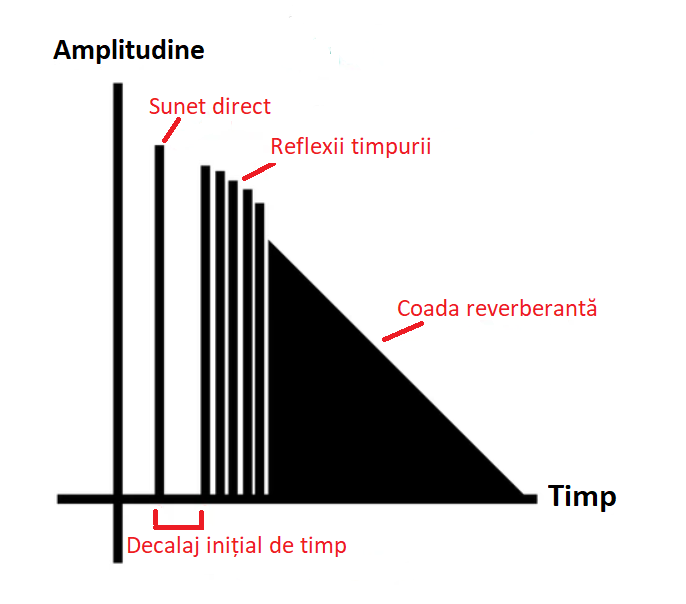
\includegraphics[width=0.7\linewidth]{imagini/impulseResponse.png}
		\caption{Func\c{t}ia de r\u{a}spuns la impuls}
		\label{Fig4}
	\end{figure}

	{\it{Sunetul direct (Direct Sound)}} are presiunea acustic\u{a} ridicat\u{a}, dar durat\u{a} scurt\u{a}, reprezent\^{a}nd timpul necesar pentru ca sunetul s\u{a} ajung\u{a} la cel primit (ex: ascult\u{a}tor sau microfon).
	 
	
	{\it{Decalaj ini\c{t}ial de timp (Initial Time Delay Gap)}}	reprezint\u{a} timpul dintre sunetul direct \c{s}i primele reflexii \c{s}i ne spune c\^{a}t de departe este sursa de sunet. Cu c\^{a}t decalajul ini\c{t}ial de timp este mai lung, cu at\^{a}t este mai apropiat\u{a} sursa de sunet. Cu alte cuvinte, dac\u{a} sursa este departe, sunetul direct \c{s}i primele reflexii se vor auzi ca și cum ar fi mai apropiate.
	 
	
	{\it{Reflec\c{t}ii timpurii (First Order Reflections sau Early Reflections)}} sunt primele pe care le auzim \c{s}i se disting. Este posibil s\u{a} fie doar c\^{a}teva \^{i}ntr-o camer\u{a} simpl\u{a} dreptunghiular\u{a}, dar pot fi mai multe dac\u{a} camera este mai complex\u{a}. Reflec\c{t}iile timpurii indic\u{a} c\^{a}t de mare este o camer\u{a}.
	 
	
	{\it{Coada reverberant\u{a}}} const\u{a} \^{i}n reflexii de ordin superior \c{s}i nu se pot distinge \^{i}ntre ele. Pe m\u{a}sur\u{a} ce num\u{a}rul de reflexii cre\c{s}te, undele sonore pierd energie \c{s}i, \^{i}n cele din urm\u{a}, se descompun. Dezintegrarea reverberant\u{a} este adesea liniar\u{a} atunci c\^{a}nd este reprezentat\u{a} grafic ca mai sus. 
	
	\section{Func\c{t}ia de r\u{a}spuns la frecven\c{t}\u{a}}
	
	Gama spectrului audio se întinde de la 20 Hz la 20.000 Hz și poate fi împărțită eficient în șapte benzi de frecvență diferite, fiecare bandă având un impact diferit asupra sunetului total. Sub-basul, cuprinde intervalul de la 20 la 60 Hz, oferă primele frecvențe joase utilizabile pe majoritatea înregistrărilor. Basul profund produs în această gamă se simte, de obicei, mai mult decât se aude, oferind un sentiment de putere. Multe instrumente se luptă să intre în acest interval de frecvență, cu excepția câtorva instrumente cu bas greu, cum ar fi chitara basă care are cel mai mic ton realizabil de 41 Hz. Este dificil de auzit gama sub-basului la volume mici datorită curbei Fletcher Munson, un contur cu intensitate egală care reprezintă o măsură a nivelului de presiune acustică, peste spectrul de frecvență, pentru care un ascultător percepe o intensitate constantă atunci când este prezentat cu tonuri stabile pure.
	
	Basul este cea de-a doua gamă și cuprinde intervalul de la 60 la 250 Hz. Notele fundamentale ale ritmului sunt centrate pe această zonă. Cele mai multe semnale de bas în piesele de muzică modernă se află în jurul zonei de 90-200 Hz. Frecvențele în jurul valorii de 250 Hz pot adăuga o senzație de căldură la bas fără pierderea definiției.
	
	Gama medie joasă conține armonicele de ordin scăzut ale majorității instrumentelor și este în general privită ca gama de prezență a basului și cuprinde valorile din intervalul 250-500 Hz. Creșterea semnalului în jurul valorii de 300 Hz adaugă claritate instrumentelor de bas și corzi inferioare. Creșterea prea mare în jurul valorii de 500 Hz poate face ca instrumentele cu frecvență mai mare să pară înăbușite.
	
	Intervalul mediu, 500 Hz - 2kHz, determină cât de proeminent este un instrument în mix. Creșterea în jur de 1000 Hz poate conferi instrumentelor o calitate asemănătoare claxonului. Excesul de ieșire la acest interval poate suna subțire și poate provoca oboseală a urechii. Dacă creșteți în acest domeniu, fiți foarte precauți, mai ales la voce. Urechea este deosebit de sensibilă la modul în care sună vocea umană și la acoperirea frecvenței acesteia.
	
	Auzul uman este extrem de sensibil la frecvențele medii ridicate, cuprinse  în intervalul 2-4kHz, cu cel mai mic impuls aici rezultând o schimbare imensă a timbrului sunetului. Gama medie înaltă este responsabilă pentru atacul asupra instrumentelor percutante și ritmice. Dacă este amplificat, acest interval poate adăuga prezență. Cu toate acestea, o creștere prea mare în jurul gamei de 3 kHz poate provoca oboseală la ascultare.
	
	Gama de prezență, 4-6 kHz, este responsabilă pentru claritatea și definirea unui sunet. Este intervalul în care majoritatea aparatelor stereo de acasă își centrează înaltele. Suprasolicitarea poate provoca un sunet iritant și dur. Tăierea în această gamă face ca sunetul să fie mai îndepărtat și mai transparent.
	
	Gama de strălucire, 6-20 kHz, este compusă în întregime din armonici și este responsabilă pentru strălucirea și aerul unui sunet. Creșterea în jurul valorii de 12 kHz face ca sunetul de înregistrare să devină mai Hi-Fi. Hi-Fi(High Fidelity) este un termen folosit de ascultători, audiofili și pasionați de sunet acasă pentru a se referi la reproducerea sunetului de înaltă calitate.

	Frecvențele mai mici de 20 Hz se numesc infrasunete, iar frecvențele care sunt mai mari de 20 kHz se numesc ultrasunete. Infrasunetele pot fi auzite și folosite de animale precum: elefanții și balenele, iar ultrasunetele sunt, de obicei, folosite în domeniul medical.
	
	\begin{figure}[!htb]
		\centering
		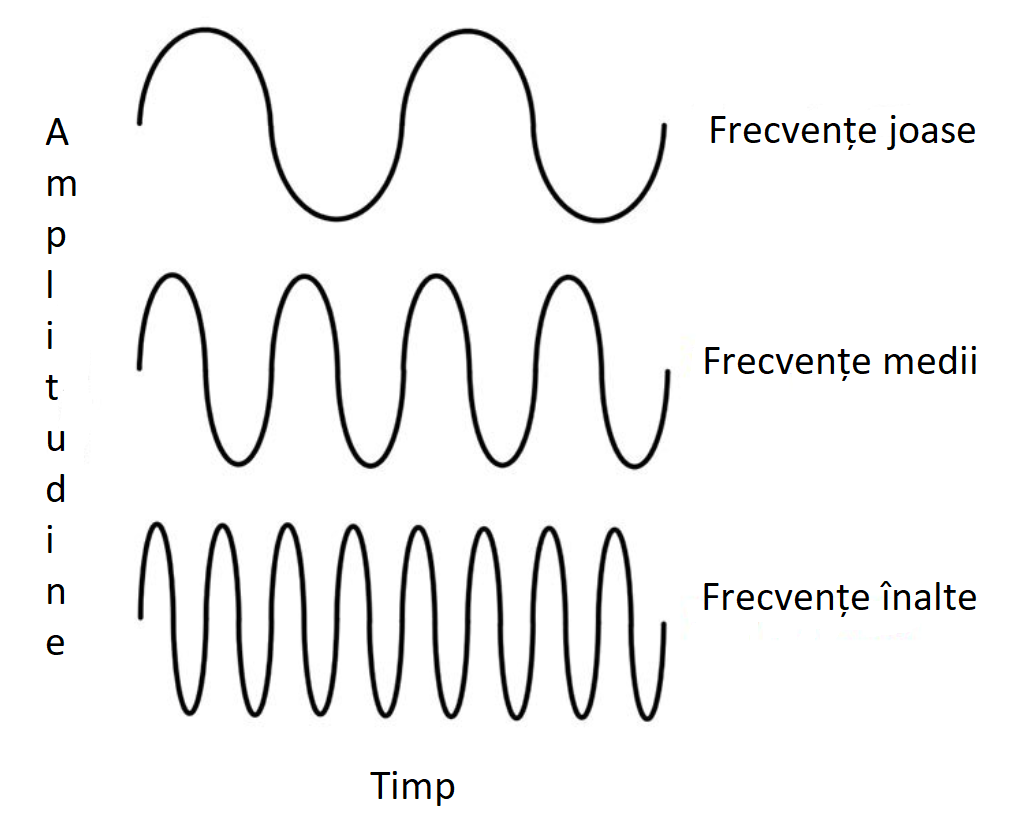
\includegraphics[width=12cm]{imagini/ampli_timp.png}
		\caption{Tipuri de frecvențe}
		\label{Fig30}
	\end{figure}

	Dacă urmăurim undele sinusoidale din Figura \ref{Fig30} putem observa că pe măsură ce crește frecvența, perioada de timp pentru un ciclu devine progresiv mai scurtă, astfel încât în comparație cu o singură perioadă de timp de $360^\circ$ la frecvență joasă, o perioadă de timp cu frecvență înaltă poate include 2 sau mai multe cicluri în aceeași perioadă de timp ca o frecvență mai mică. Astfel, avem ilustrate frecvențele joase, medii și înalte în funcție de amplitudine și timp.
	
	Răspunsul în frecvență este măsura cantitativă a spectrului de ieșire al unui sistem sau dispozitiv ca răspuns la un stimul și este utilizat pentru a caracteriza dinamica sistemului. Este o măsură a magnitudinii și a fazei în funcție de frecvență, în comparație cu intrarea. În termeni simpli, dacă o undă sinusoidală este injectată într-un sistem la o frecvență dată, un sistem liniar va răspunde la aceeași frecvență cu o anumită magnitudine și un anumit unghi de fază relativ la intrare.	 
	
	\^{I}n contextul unui sistem audio, obiectivul poate fi reproducerea semnalului de intrare f\u{a}r\u{a} distorsiuni. Acest lucru necesit\u{a} o amplitudine de r\u{a}spuns uniform p\^{a}n\u{a} la limitarea l\u{a}\c{t}imii de band\u{a} a sistemului, cu semnalul \^{i}nt\^{a}rziat cu exact aceea\c{s}i cantitate de timp la toate frecven\c{t}ele.	 
	
	Estimarea r\u{a}spunsului \^{i}n frecven\c{t}\u{a} pentru un sistem fizic implic\u{a}, \^{i}n general, excitarea semnalului cu un semnal de intrare, m\u{a}surarea istoricelor de timp de intrare \c{s}i de ie\c{s}ire \c{s}i compararea celor dou\u{a} printr-un proces precum Transformarea Fourier Rapid\u{a} (FFT).
	
	R\u{a}spunsul \^{i}n frecven\c{t}\u{a} se caracterizeaz\u{a} prin amploarea r\u{a}spunsului sistemului, m\u{a}surat\u{a}, de obicei, \^{i}n decibeli (dB), \c{s}i faza, m\u{a}surat\u{a} \^{i}n radiani sau grade. Funcția de răspunsul în frecvență are, în general, valori complexe, cu părți reale și imaginare. Acest lucru este adesea mai util și mai intuitiv atunci când este exprimat în coordonate polare. Adică îl putem separa în magnitudinea sa (numită răspuns de amplitudine) și în componentă de fază (numită răspuns de fază).
	
	Fiecare componentă din semnal ar trebui să aibă, în mod ideal, un răspuns de frecvență plat, astfel încât sunetul să treacă nealterat. Dar realitatea este că multe componente nu oferă performanțe ideale. Un răspuns neliniar va modifica modul în care sună sursa noastră. Cu toate acestea, nu este vorba doar de concepte obișnuite, cum ar fi basul și înalte, ci afectează și calitatea sunetului fiecărui instrument din mix. Pentru a ne pune capul în jurul acestui aspect mai subtil al modului în care răspunsul de frecvență neliniar poate afecta ceea ce auzim, trebuie să apelăm la analiza Fourier.
	
	\section{Absorb\c{t}ia sunetului}
	
	\^{I}n contextul propag\u{a}rii sunetului \^{i}n spa\c{t}ii \^{i}nchise vom considera dou\u{a} tipuri de absorb\c{t}ii: \textit{absorb\c{t}ia aerului} \c{s}i \textit{absorb\c{t}ia suprafe\c{t}elor}.
	 
	
	\textit{Coeficientul de absorb\c{t}ie \^{i}n aer}, depinde de temperatura atmosferic\u{a}, de presiunea atmosferic\u{a} \c{s}i de frecven\c{t}\u{a}. Absorb\c{t}ia sunetului \^{i}n acustic\u{a} este cauzat\u{a} de caracteristicile de absorb\c{t}ie ale suprafe\c{t}elor. Atunci când ținem cont de absorbția aerului putem îmbunătății rezultatele pentru încăperile de dimensiuni mari sau atunci când considerăm frecvențe înalte.
	
	Astfel, absorb\c{t}ia este definit\u{a} ca o disipare a energiei sonore la lovirea unei suprafe\c{t}e fizice. La fiecare reflexie, o parte $\alpha$ din energia sau puterea sa este absorbit\u{a}. Acest factor $\alpha$ se nume\c{s}te coeficient de absorb\c{t}ie. Absorb\c{t}ia sunetului depinde de unghiul de inciden\c{t}\u{a}.
	
	În solide și lichide se absoarbe mai puțin sunet decât în gaze, sunetele se pot propaga pe distanțe mult mai mari în aceste medii. De exemplu, marea gamă pe care pot comunica anumite mamifere marine este posibilă parțial prin atenuarea redusă a sunetului în apă. În plus, deoarece absorbția crește odată cu frecvența, devine foarte dificil ca undele ultrasonice să pătrundă într-un mediu dens. Aceasta este o limitare persistentă a dezvoltării aplicațiilor cu ultrasunete de înaltă frecvență.
	
	Un alt mecanism de absorb\c{t}ie a sunetului este \textit{absorb\c{t}ia suprafe\c{t}elor}, fiind definit ca disiparea energiei sonore la lovirea unei suprafe\c{t}e fizice. La fiecare reflexie, o parte din energie sau putere este absorbit\u{a}. Restul de energie care nu este absorbit\u{a} este fie absorbit\u{a} de material, fie transmis\u{a} mai departe ca sunet reflectat. Formula utilizat\u{a} \^{i}n aceast\u{a} lucrare este eviden\c{t}iat\u{a} prin Ecuatia \eqref{ecuatia3}.
	
	\begin{equation}
		W = W(1-\alpha)
		\label{ecuatia3}
	\end{equation}
	
	\noindent unde $W$ este energia.
	
	Absorbția sunetului nedorit, precum cel al mașinilor din fabrici, este esențială pentru sănătatea lucrătorilor, iar controlul zgomotului în acustica arhitecturală și industrială s-a extins pentru a deveni un domeniu important al ingineriei acusticii.
	
	Materialele de absorbție a sunetului sunt utilizate pe scară largă în multe aplicații de control al zgomotului. Comportamentul acustic al acestor materiale poate fi măsurat folosind tubul de impedanță cu eșantioane de dimensiuni mici, dar în practică, materialele utilizate în aplicațiile de control al zgomotului nu sunt mici, iar undele incidente de pe acestea nu sunt unde plane. În practică, materiale în diferite dimensiuni și forme sunt utilizate în aplicații de control al zgomotului, iar câmpul acustic este difuz. Impedanța acustică este o măsură a ușurinței cu care o undă sonoră se propagă printr-un anumit mediu.
	
	Coeficientul de absorbție reprezintă raportul dintre energia absorbită de suprafață și energia incidentă. Conform definiției sale, coeficientul de absorbție a sunetului unei suprafețe poate presupune valori cuprinse între 0 (suprafețe care reflectă total) și 1 (suprafețe absorbante total).
	
	Calitatea acustică a unei camere depinde de reverberație, care la rândul ei este direct proporțională cu volumul camerei și invers proporțională cu capacitatea de a absorbi sunetul materialelor limită și a tuturor celorlalte obiecte plasate în interiorul camerei.
	
	În această lucrare se va ține cont doar de coeficientul de absorbție al suprafețelor.
	
	\section{Simularea binaural\u{a}}
	
	\textit{Simularea binaural\u{a}} reprezint\u{a} o metod\u{a} de a realiza semnale binaurale la ambele urechi ale receptorului \^{i}n spa\c{t}ii inexistente prin intermediul unui model. \^{I}n ultima perioad\u{a}, simularea acustic\u{a} a devenit din ce \^{i}n ce mai important\u{a} pentru proiectarea spa\c{t}iilor \^{i}nchise, precum s\u{a}lile de concerte \c{s}i de teatru.
	 
	
	Exist\u{a} o mul\c{t}ime de tehnici de simulare binaural\u{a} \^{i}n combina\c{t}ie cu metode de calcul, de cele mai multe ori tehnici geometrice pentru calcul acustic, precum: metoda sursei de imagine \^{i}n oglind\u{a}, ray-tracing sau metode hibride. Cu toate acestea, genul acesta de tehnici vin la pachet cu cre\c{s}terea timpului de calcul. Unul dintre cele mai dificile lucruri este directivitatea sursei.
	
	 
	De\c{s}i este imposibil\u{a} simularea cu exactitate a unui c\^{a}mp sonor real folosind metode geometrice, lucr\u{a}rile realizate p\^{a}n\u{a} \^{i}n prezent pe aceste teme s-au bucurat de un mare succes, iar unele au fost chiar comercializate. O alt\u{a} provocare \^{i}n crearea unui astfel de algoritm este dat\u{a} de coada reverberant\u{a} datorit\u{a} efortului considerabil de timp. Simularea binaural\u{a} nu va fi tratat\u{a} \^{i}n acest studiu.
	
	\begin{figure}[!htb]
		\centering
		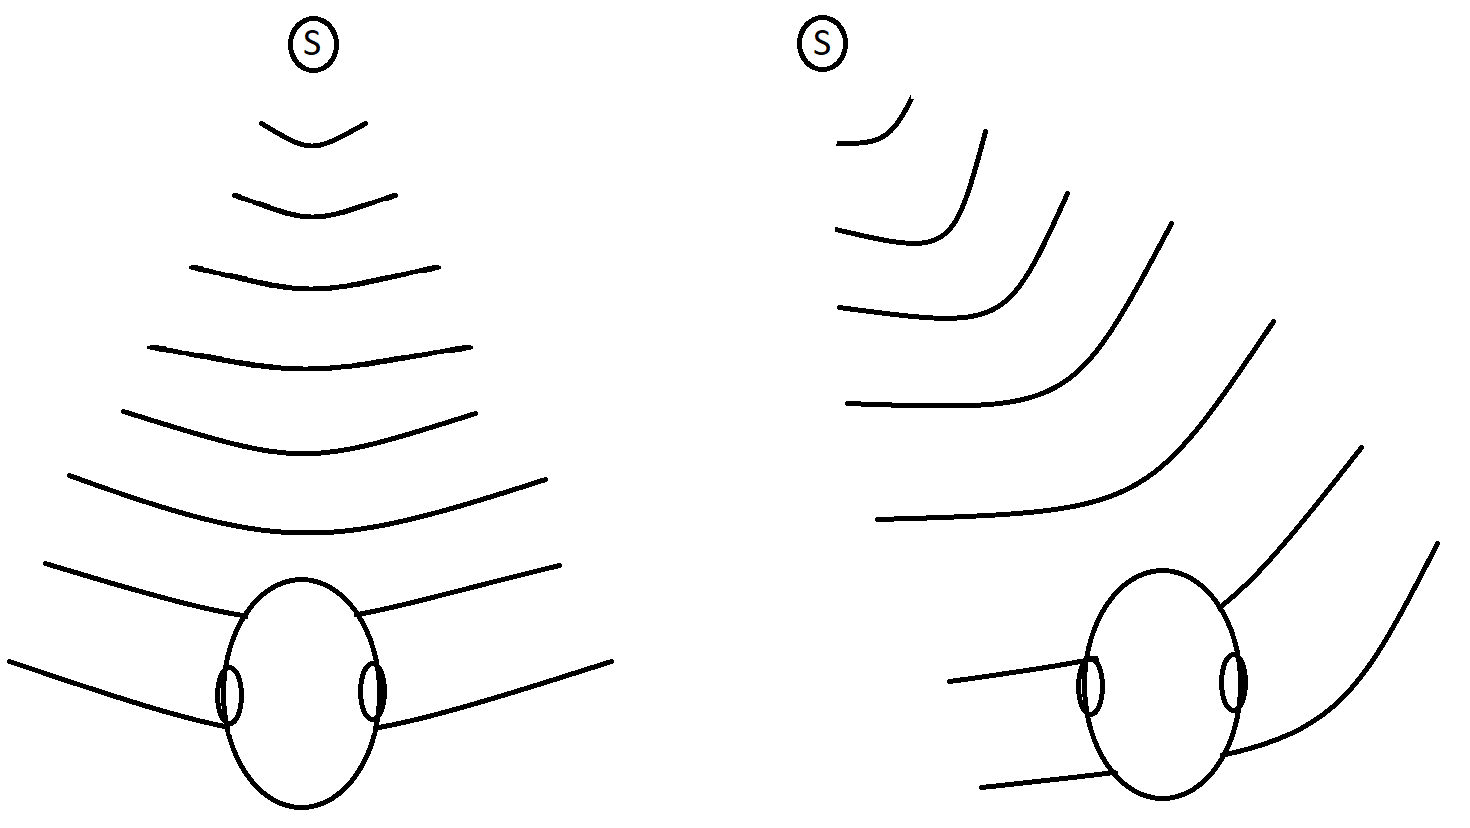
\includegraphics[width=1\linewidth]{imagini/binauralExample.png}
		\caption{Exemplu de simulare binaural\u{a}}
		\label{Fig12}
	\end{figure}

	\^{I}n Figura \ref{Fig12}, se poate observa beneficiul unei simul\u{a}ri binaurale. \^{I}n prima parte a figurii, sunetul ajunge de la surs\u{a} (S) la urechile omului \^{i}n acela\c{s}i moment \c{s}i cu aceea\c{s}i intensitate, pe c\^{a}nd \^{i}n partea din dreapta imaginii sunetul ajunge mai devreme la urechea st\^{a}ng\u{a} dec\^{a}t la urechea dreapt\u{a} \c{s}i la intensit\u{a}\c{t}i diferite. Urechea st\^{a}ng\u{a} va auzi mai puternic sunetul dec\^{a}t urechea dreapt\u{a}. 

	\section{Tehnica de trasare a razelor (Ray-Tracing)}
	
	Intensitatea emis\u{a} de o surs\u{a} este descris\u{a} de un num\u{a}r finit de raze, care vor fi considerate purt\u{a}tori de intensitate (sau de energie sau de putere). Aceste raze c\u{a}l\u{a}toresc prin spa\c{t}iu la viteza sunetului \c{s}i sunt reflectate dup\u{a} fiecare coliziune cu limitele camerei. \^{I}n acest timp, intensitatea lor scade ca o consecin\c{t}\u{a} a absorb\c{t}iei aerului \c{s}i a pere\c{t}ilor pe care raza \^{i}i intersecteaz\u{a}.
	 
	
	Dac\u{a} sursa sonor\u{a} are caracteristici omnidirec\c{t}ionale, direc\c{t}iile razelor sunt create prin distribu\c{t}ii aleatoare omogene. Calea posibil\u{a} pentru fiecare raz\u{a} emis\u{a} de la surs\u{a} trebuie gasit\u{a}. Raza este considerat\u{a} un vector care \^{i}\c{s}i schimb\u{a} direc\c{t}ia la fiecare reflexie, fiind astfel posibil\u{a} determinarea urm\u{a}toarei suprafe\c{t}e de ciocnire. 
	 
	
	De obicei, sursa este \^{i}mp\u{a}r\c{t}it\u{a} \^{i}ntr-un num\u{a}r mare de piese mici. Metoda determinist\u{a} este \^{i}mp\u{a}r\c{t}irea sursei \^{i}ntr-o manier\u{a} matematic\u{a} sau geometric\u{a}. Piesele din surs\u{a} ar trebui s\u{a} fie identice sau c\^{a}t de mult posibil identice. Punctele selectate aleatoriu pe suprafa\c{t}a unei sfere surs\u{a} pot fi reprezentate de trei parametrii: raza, azimutul \c{s}i eleva\c{t}ia \cite{jeong}. Mai mult dec\^{a}t a propus Jeong Cheol-Ho \^{i}n studiul s\u{a}u, \^{i}n aceast\u{a} lucrare \^{i}mp\u{a}r\c{t}irea sursei \^{i}n piese mai mici s-a realizat cu ajutorul sferei lui Fibonacci, algoritm ce urmeaz\u{a} s\u{a} fie descris \^{i}n capitolele urm\u{a}toare.
	 
	
	Mai departe, aceste puncte reprezint\u{a} pozi\c{t}ia de start pentru o raz\u{a}. Fiecare raz\u{a} poate avea nici una sau mai multe reflexii \c{s}i, astfel, s\u{a} fie considerat\u{a} o raz\u{a} direct\u{a} sau indirect\u{a}. Fiecare coliziune este re\c{t}inut\u{a} \c{s}i putem observa care a fost traseul pe care fiecare raz\u{a} l-a parcurs \^{i}n \^{i}nc\u{a}pere de la surs\u{a} p\^{a}n\u{a} la ascult\u{a}tor.
	 
	
	Intensitatea pe care o raz\u{a} o transmite receptorului este direct dependent\u{a} de distan\c{t}a pe care raza a parcurs-o \^{i}n \^{i}nc\u{a}pere. Intensitatea la un anumit moment se calculeaz\u{a} astfel dependent de absorb\c{t}ia aerului, de lungimea traseului parcurs \c{s}i de propriet\u{a}\c{t}ile de absorb\c{t}ie ale peretelui. Coliziunea cu suprafa\c{t}a poate fi considerat\u{a} specular\u{a}, conform legii lui Snell.	Tot acest proces trebuie repetat pentru fiecare frecven\c{t}\u{a}.
	 
	
	\^{I}n Figura \ref{Fig9} este ilustrat un mod de reprezentare pentru tehnica Ray-Tracing, unde se poate observa traiectul razelor. Linia continu\u{a} reprezint\u{a} raza direct\u{a}, iar liniile punctate semnific\u{a} razele indirecte.
	
	\begin{figure}[!htb]
		\centering
		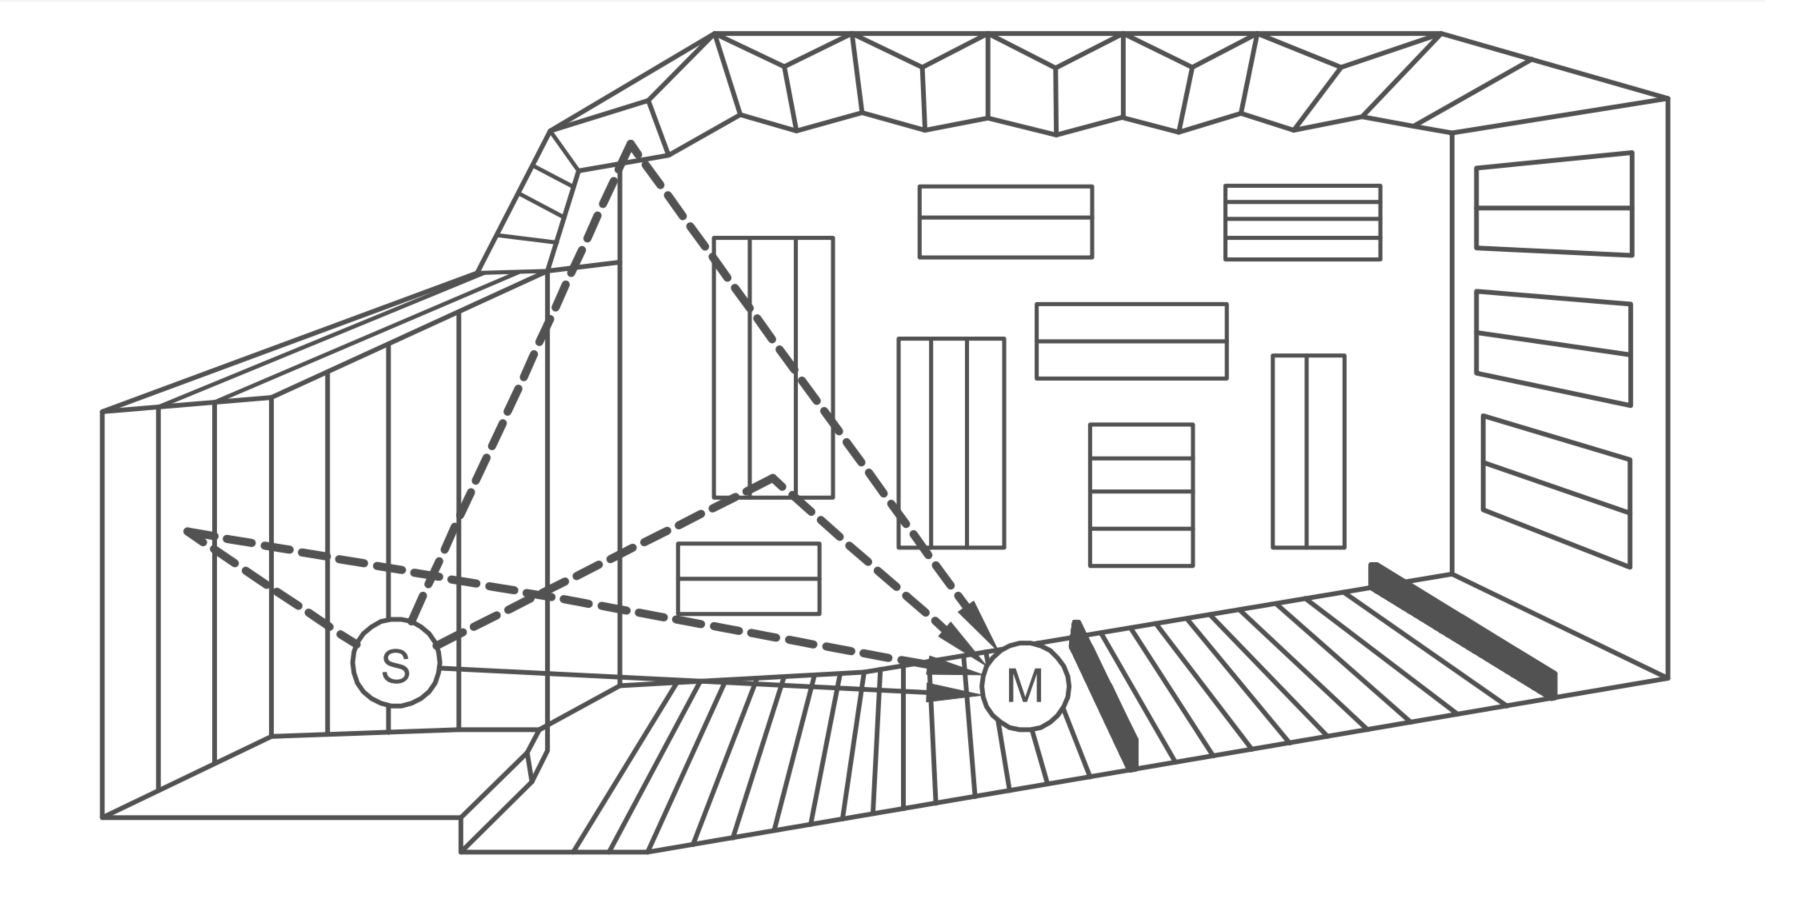
\includegraphics[width=1\linewidth]{imagini/roomExample.png}
		\caption{Exemplu de ray-tracing}
		\label{Fig9}
	\end{figure}
	
	S-a demonstrat c\u{a} algoritmul de Ray-Tracing prezice nivelurile de zgomot cu o precizie foarte bun\u{a} \c{s}i este considerat drept unul dintre cele mai elegante metode de reprezentare a reflexiilor. Cu toate acestea, exist\u{a} limit\u{a}ri, excep\c{t}ii \c{s}i probleme. Exist\u{a} c\^{a}teva elemente care ar trebui luate \^{i}n considerare atunci c\^{a}nd implement\u{a}m sau evalu\u{a}m un astfel de algoritm, precum: \textit{intervalul de frecven\c{t}e}, \textit{factori dependen\c{t}i de frecven\c{t}\u{a}}, \textit{geometria}, \textit{num\u{a}rul de raze}.
	 
	
	\^{I}n mod normal, singurii factori dependen\c{t}i de frecven\c{t}\u{a} care pot fi inclu\c{s}i sunt coeficien\c{t}ii de absorb\c{t}ie \c{s}i estimarea statistic\u{a} a propriet\u{a}\c{t}ilor difuze. O ipotez\u{a} de baz\u{a} \^{i}n metodele care utilizeaz\u{a} raze este c\u{a} lungimea de und\u{a} corespunz\u{a}toare celei mai mici frecven\c{t}e este mai mic\u{a} \^{i}n compara\c{t}ie cu dimensiunile camerei \c{s}i suprafe\c{t}ele acesteia.
	 
	
	Precum am men\c{t}ionat mai sus, coeficientul de absorb\c{t}ie $\alpha$ este dependent de unghi. Principalul motiv pentru evitarea m\u{a}sur\u{a}torilor dependente de unghi este c\u{a} acestea ar trebui s\u{a} fie foarte precise. Acest lucru fiind destul de dificil, \^{i}ntruc\^{a}t presupune stocarea tuturor materialelor de construc\c{t}ie. Prin urmare, a fost acceptat\u{a} estimarea caracteristicilor de absorb\c{t}ie a unei suprafe\c{t}e printr-o form\u{a} care este \^{i}n medie peste toate unghiurile de inciden\c{t}\u{a}.
	 
	
	Erori numerice sunt introduse \^{i}n rezultate prin utilizarea unui num\u{a}r limitat de raze, deoarece unghiul dintre raze adiacente r\u{a}m\^{a}ne constant, iar aceast\u{a} reprezentare devine treptat mai pu\c{t}in exact\u{a} odat\u{a} cu sc\u{a}derea num\u{a}rului de raze. Pentru a atinge criteriile de convergen\c{t}\u{a}, num\u{a}rul de raze trebuie s\u{a} fie c\^{a}t mai mare, cu c\^{a}t num\u{a}rul de raze este mai mare, cu at\^{a}t este mai mic unghiul solid pe care \^{i}l va acoperi o raz\u{a}. Acest lucru poate afecta timpul de calcul, dar \c{s}i un num\u{a}r prea mic de raze poate genera probleme. 
	 
	
	Pentru a putea \^{i}n\c{t}elege mai bine traiectul unei raze vom folosi Figura \ref{Fig11}. S \c{s}i M reprezint\u{a} sursa \c{s}i microfonul, iar linia trasat\u{a} este drumul parcurs de raz\u{a} p\^{a}n\u{a} la microfon, drum care presupune 4 reflexii speculare. Modelul de propagare al sunetului ce urmeaz\u{a} s\u{a} fie prezentat \^{i}n aceast\u{a} lucrare va folosi doar reflexii speculare.
	 
	
	\begin{figure}[!htb]
		\centering
		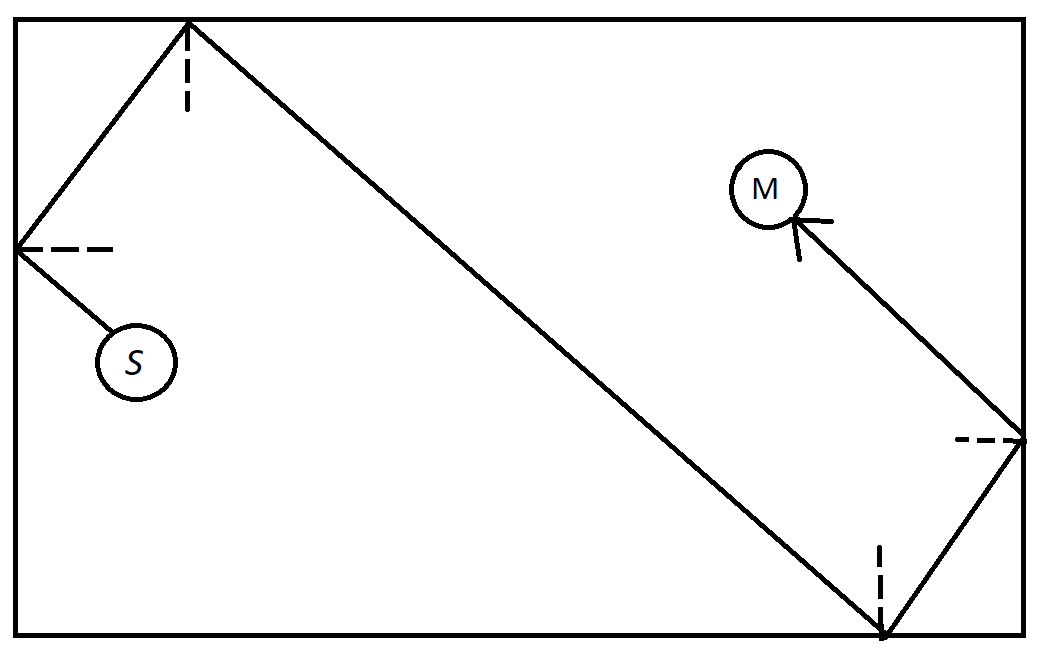
\includegraphics[width=1\linewidth]{imagini/reflectionExample.png}
		\caption{Calea unei raze de la surs\u{a} la microfon}
		\label{Fig11}
	\end{figure}
	
	Atunci c\^{a}nd se dore\c{s}te implementarea unui algoritm de acest gen, exist\u{a} c\^{a}\c{t}iva factori foarte importan\c{t}i c\^{a}nd ne g\^{a}ndim la timpul de calcul, precum: num\u{a}rul de raze, lungimea maxim\u{a} pe care o raz\u{a} o poate avea, num\u{a}rul maxim de reflexii pe care \^{i}l poate avea o raz\u{a}, chiar \c{s}i procesorul pe care \^{i}l are ma\c{s}ina de pe care lucr\u{a}m poate influen\c{t}a semnificativ timpul de calcul.
	 
	
	Astfel, realizarea unui algoritm care modeleaz\u{a} acustic spa\c{t}iile \^{i}nchise presupune dou\u{a} mari etape: realizarea unui model geometric \c{s}i implementarea unui model fizic. Prima etap\u{a} se ocup\u{a} de definirea dimensiunilor \^{i}nc\u{a}perii, a\c{s}ezarea sursei \c{s}i a microfoanelor \^{i}n spa\c{t}iu, trasarea razelor \c{s}i determinarea razelor intersectate cu microfoanele. A doua etap\u{a} presupune calcularea m\u{a}surilor fizice: intensitatea, presiunea, faza, magnitudinea, func\c{t}ia de r\u{a}spuns la impuls și funcția de răspuns în frecvență. 
	
	\section{Convolu\c{t}ia sunetului}
	
	Convolu\c{t}ia în domeniul timpului înseamnă că spectrele sunt multiplicate. Prin „multiplicarea” spectrelor înțelegem că orice frecvență care este puternică în ambele semnale va fi foarte puternică în semnalul convolut și invers orice frecvență care este slabă în ambele semnale de intrare va fi slabă în semnalul de ieșire. Convolu\c{t}ia implic\u{a} dou\u{a} func\c{t}ii matematice $f$ \c{s}i $g$ care produc o a treia func\c{t}ie $h$ ce reprezint\u{a} modul \^{i}n care forma uneia este modificat\u{a} de c\u{a}tre cealalt\u{a}.
	 
	
	Atunci c\^{a}nd vorbim despre convolu\c{t}ie, sursa de sunet este numit\u{a} semnal de intrare, iar fi\c{s}ierul de ie\c{s}ire este r\u{a}spunsul la impuls. Fi\c{s}ierul de r\u{a}spuns la impuls are mereu o lungime fix\u{a}.
	 
	
	În practică, o aplicare relativ simplă a convoluției este locul în care avem „func\c{t}ia de răspunsul la impuls” al unui spațiu. Acest lucru se obține înregistrând o scurtă explozie a unui semnal de bandă largă pe măsură ce este procesat de caracteristicile reverberante ale spațiului. Cu alte cuvinte, a fost procesat de func\c{t}ia de răspuns în frecvență al spațiului similar cu modul în care ar funcționa acest proces în spațiul real. De fapt, convoluția din acest exemplu este pur și simplu o descriere matematică a ceea ce se întâmplă atunci când orice sunet este ,,colorat" de spațiul acustic în care apare, ceea ce este de fapt adevărat pentru toate sunetele din toate spațiile, cu excepția unei camere anecoice. O cameră anecoică este o cameră proiectată pentru a absorbi complet reflexiile undelor sonore sau electromagnetice. De asemenea, ele sunt adesea izolate de valurile care intră din împrejurimile lor. Această combinație înseamnă că o persoană sau un detector aude exclusiv sunete directe (fără sunete reverberante), de fapt simulând că se află într-o cameră infinit de mare. Sunetul convolut va apărea, de asemenea, la aceeași distanță ca în înregistrarea originală a impulsului. Dacă convolu\c{t}ion\u{a}m un sunet de două ori cu același răspuns la impuls, distanța sa aparentă va fi de două ori mai mare.
	 
	
	Teorema de bază despre domeniul timpului și domeniul frecvenței este că multiplicarea într-un domeniu este echivalentă cu convoluția din celălalt domeniu.
	 
	
	În cele din urmă, există o diferență tehnică între \textit{convoluție directă}, care este un proces foarte lent, dat fiind că fiecare eșantion din fiecare semnal trebuie să fie multiplicat cu fiecare eșantion din celălalt semnal. O variant\u{a} mai rapid\u{a} de a face acest lucru este folosirea Transformatei Rapide Fourier si folosirea Inversei Transofrmatei Rapide Fourier.
	 
	
	\^{I}n practic\u{a}, convolu\c{t}ia se realizeaz\u{a} cel mai adesea prin calculul FFT sau analizele spectrale pentru fi\c{s}ierele de intrare \c{s}i r\u{a}spunsul la impuls, \^{i}nmul\c{t}ind spectrele lor \^{i}mpreun\u{a}. Aceasta se nume\c{s}te  \textit{convolu\c{t}ie rapid\u{a}}. Scopul analizei spectrale este de a afla cum se distribuie energia acustică în funcție de frecvență. Crearea unei spectrograme utilizând FFT este un proces digital. Datele eșantionate digital, în domeniul timpului, sunt împărțite în bucăți, care de obicei se suprapun, și transformata Fourier pentru a calcula magnitudinea spectrului de frecvență pentru fiecare bucată. Fiecare bucată corespunde apoi unei linii verticale din imagine. Aceste spectre sau grafice de timp sunt apoi „așezate una lângă alta” pentru a forma imaginea.
	
	\section{Transformata Rapid\u{a} Fourier \c{s}i Inversa Transformatei Rapide Fourier}
	
	Transformata Fourier Rapid\u{a} (FFT) este un algoritm care calculeaz\u{a} transformata direct\u{a} (DFT) a unei secven\c{t}e sau inversa acesteia (IDFT). Analiza Fourier converte\c{s}te un semnal din domeniul timpului sau al spa\c{t}iului \^{i}n domeniul frecven\c{t}elor \c{s}i invers.
	 
	
	Transformata Fourier Discret\u{a} (DFT) transform\u{a} o secven\c{t}\u{a} de $N$ numere complexe ${x_n} = x_0, x_1, \dots, x_{N-1}$ \^{i}ntr-o alt\u{a} secven\c{t}\u{a} de numere complexe ${X_k} = X_0, X_1, \dots, X_{N-1}$ \c{s}i are urm\u{a}toarea formul\u{a} \cite{fft}:
	\begin{equation}
		X_k = \sum_{n=0}^{N-1}x_n \cdot e^{-\dfrac{i2\pi}{N}kn}
	\end{equation}
	 
	
	DFT este o opera\c{t}ie foarte util\u{a}, dar destul de costisitoare, din acest motiv a ap\u{a}rut FFT, care calculeaz\u{a} rapid astfel de transform\u{a}ri factoriz\^{a}nd matricea DFT \^{i}ntr-un produs de factori rari (\^{i}n mare parte zero). \^{I}n acest mod, complexitatea algoritmului este redus\u{a} de la $O(N^2)$ la $O(N\lg N)$. Diferența de viteză poate fi enormă, în special pentru seturile de date lungi, unde $N$ poate de ordinul miilor sau milioanelor. În prezența unei erori de rotunjire, mulți algoritmi FFT sunt mult mai exacți decât evaluarea definiției DFT direct sau indirect.
	 
	Transformata Fourier este utilizată pentru analiza spectrală a seriilor temporale. Cu toate acestea, subiectul procesării statistice a semnalului nu aplică, de obicei, Transformata Fourier asupra semnalului însuși. Chiar dacă un semnal real este într-adevăr tranzitoriu, s-a găsit în practică recomandabil modelarea unui semnal printr-o funcție ale cărei caracteristici sunt constante de-a lungul timpului Transformata Fourier a unei astfel de funcții nu există în sensul obișnuit și s-a considerat utilă pentru analiza semnalelor.

	Reprezentarea \^{i}n domeniul frecven\c{t}\u{a} presupune descopunerea unui semnal acustic \^{i}n semnale sinusoidale caracterizate prin frecven\c{t}\u{a}, amplitudine \c{s}i faz\u{a}. FFT permite modificarea semnalului prin atenuare/eliminare de frecven\c{t}e - filtrare \^{i}n domeniul frecven\c{t}\u{a}.
	 
	
	Pentru a atinge performan\c{t}e exist\u{a} mai mul\c{t}i algoritmi care calculeaz\u{a} FFT, iar ace\c{s}ti algoritmi, de obicei, presupun \^{i}mpar\c{t}irea polinomului ini\c{t}ial \^{i}n dou\u{a} polinoame. Polinomul calculat poate fi caracterizat de r\u{a}d\u{a}cinile complexe conjugate prin r\u{a}d\u{a}cini de ordin $N$ ale unit\u{a}\c{t}ii. Acest polinom trebuie evaluat la doar $\dfrac{N}{2}$ r\u{a}d\u{a}cini ale unit\u{a}\c{t}ii. Una dintre condi\c{t}iile necesare pentru a atinge aceste performan\c{t}e de viteze este ca $N$ s\u{a} fie o putere de-a lui 2.
	
	Principala proprietate a Transformatei Fourier este aceea că transformă o funcție de timp, $x(t)$, unde $t$ reprezintă timpul, într-o funcție în frecvență $\omega$. Vom defini funcția de răspuns în frecvență astfel:
	
	\begin{equation}
		W(j\omega)= \frac{1}{(j\omega)^2m+j\omega c + k}=\frac{1}{k-m\omega^2+j\omega c}
	\end{equation}

	După cum se poate observa, funcția de răspuns în frecvență poate fi rescrisă ca un număr complex de forma:
	
	\begin{equation}
		W(j\omega)=Re(\omega)+jIm(\omega)=A(\omega)e^{j\phi \omega}
	\end{equation}
	
	\noindent unde $Re(\omega)$ este partea reală, $Im(\omega)$ este partea imaginară, $A(\omega)$ este modul și $\phi$ este faza funcției de transfer de frecvență. Componentele $Re(\omega)$, $Im(\omega)$, $A(\omega)$ și $\phi(\omega)$ se numesc caracteristicile funcției de răspuns în frecvență.
	
	\begin{figure}[!htb]
		\centering
		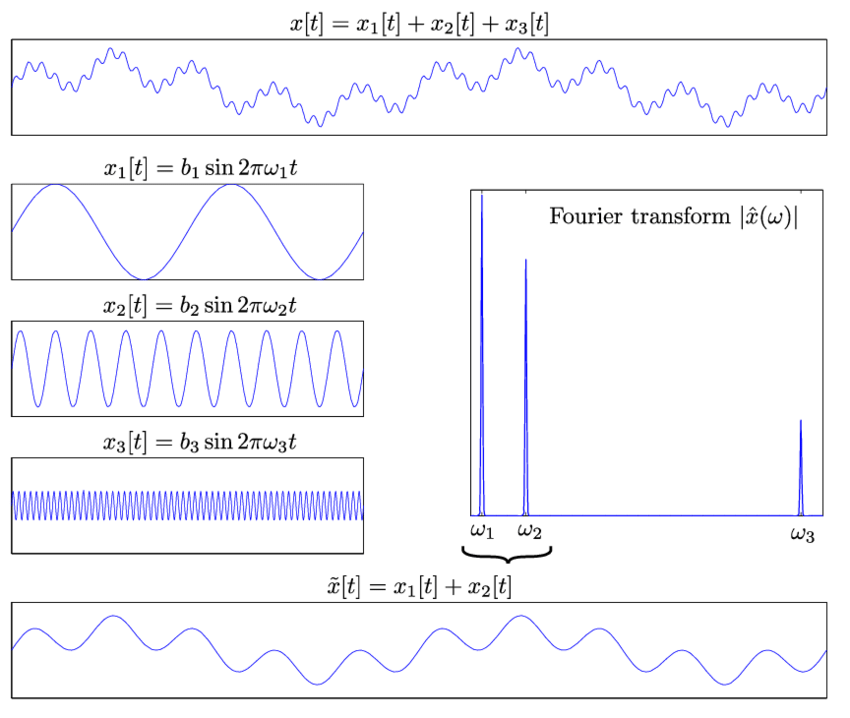
\includegraphics[width=15cm]{imagini/fft.png}
		\caption{Exemplu de transformare al semnalului cu ajutorul Transformatei Rapide Fourier}
		\label{Fig14}
	\end{figure}
	
	\^{I}n Figura \ref{Fig14}, putem observa trei semnale $x_1, x_2, x_3$ care \^{i}mpreun\u{a} formeaz\u{a} semnalul $x$ \c{s}i sunt transformate cu ajutorul Transformatei Rapide Fourier pentru a compune semnalul transformat. 
	
	Analiza Fourier și transformata Fourier dezvăluie că o formă de undă complexă poate fi exprimată ca suma unei serii de unde sinusoidale de amplitudini diferite. Deci un pătrat, triunghi sau orice altă formă de undă care apare în domeniul timpului poate fi reprezentată de mai multe frecvențe individuale diferite de amplitudini variabile în domeniul frecvenței. Aceasta include formele undelor create de instrumentele muzicale, variind de la bătăile ascuțite ale unui tambur până la chitarele electrice cu undă pătrată.
	